\section{Results}
\label{sec:results}

Figure \ref{fig:main_result} shows the results from the experiments. Figure \ref{fig:original_result} shows the results from the original paper. This section examines the results from this project and compares them to the original. All of the experiments were run three times to evaluate the variation in performance of the ablations. 

\begin{figure}[H]
    \centering
    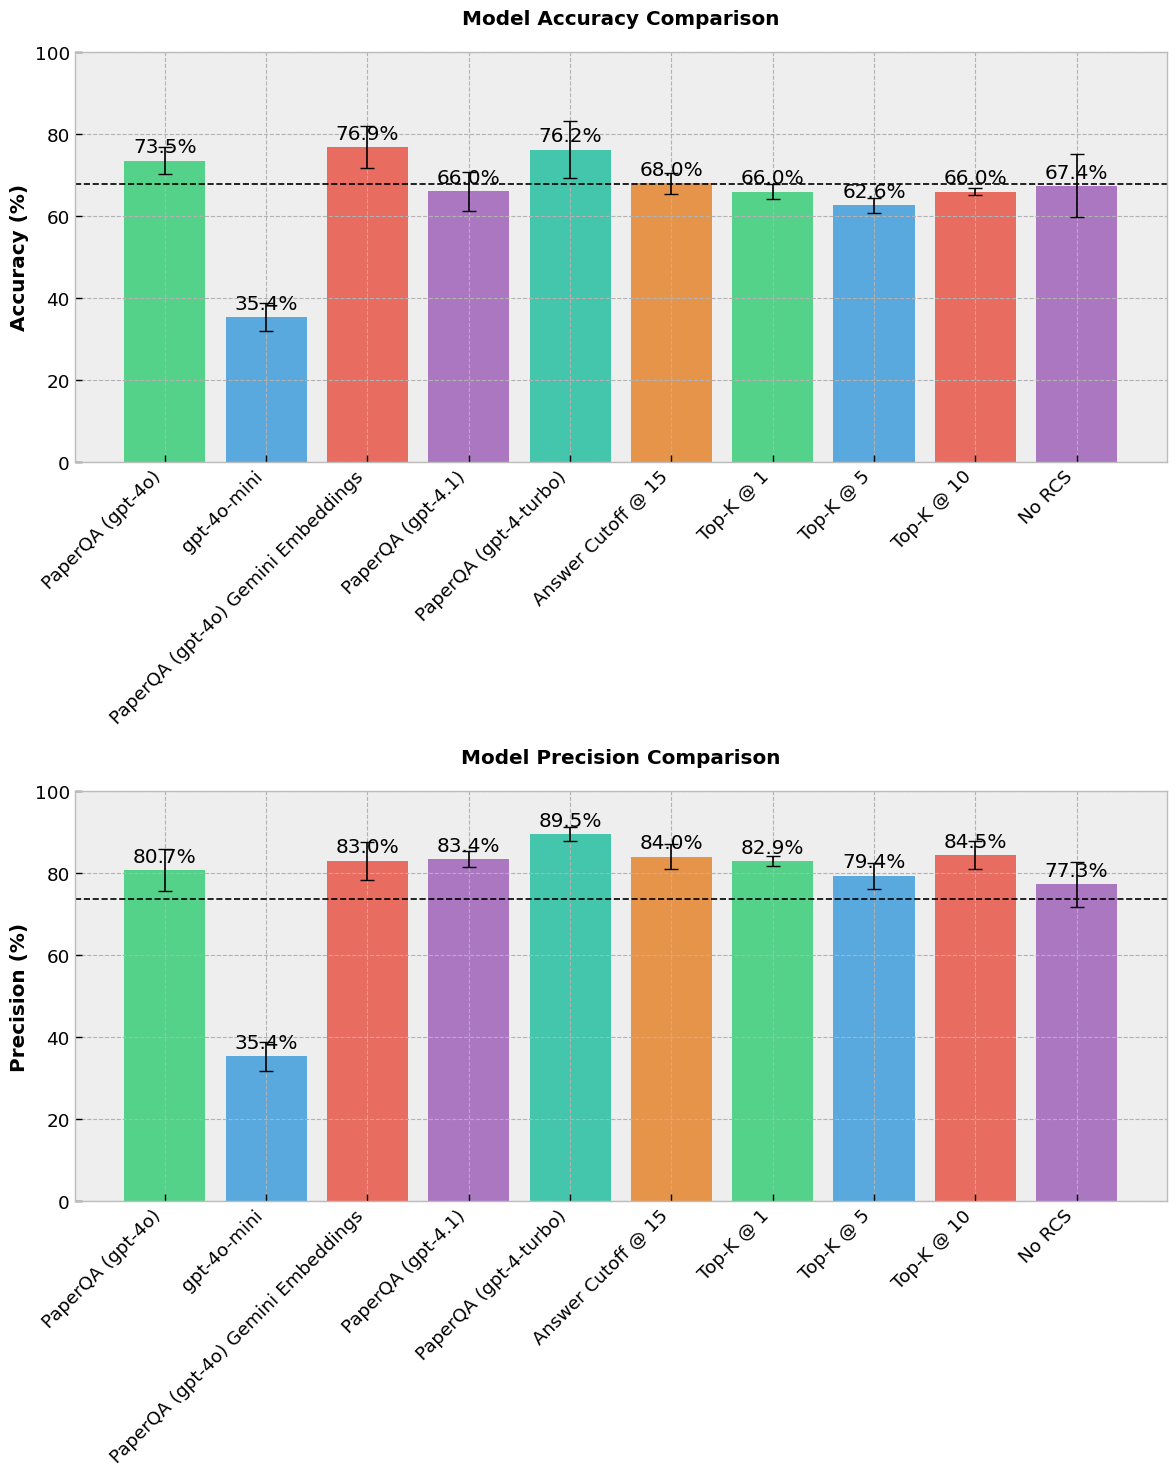
\includegraphics[width=\textwidth]{figures/main_result.png}
    \caption{This project's results against the LitQA test set. Top: Average accuracy of various setups of PaperQA. Bottom: Average precision of the various setups of PaperQA. The dashed line in each plot represents the human benchmark for both accuracy and precision.}
    \label{fig:main_result}
\end{figure}

\begin{figure}[H]
    \centering
    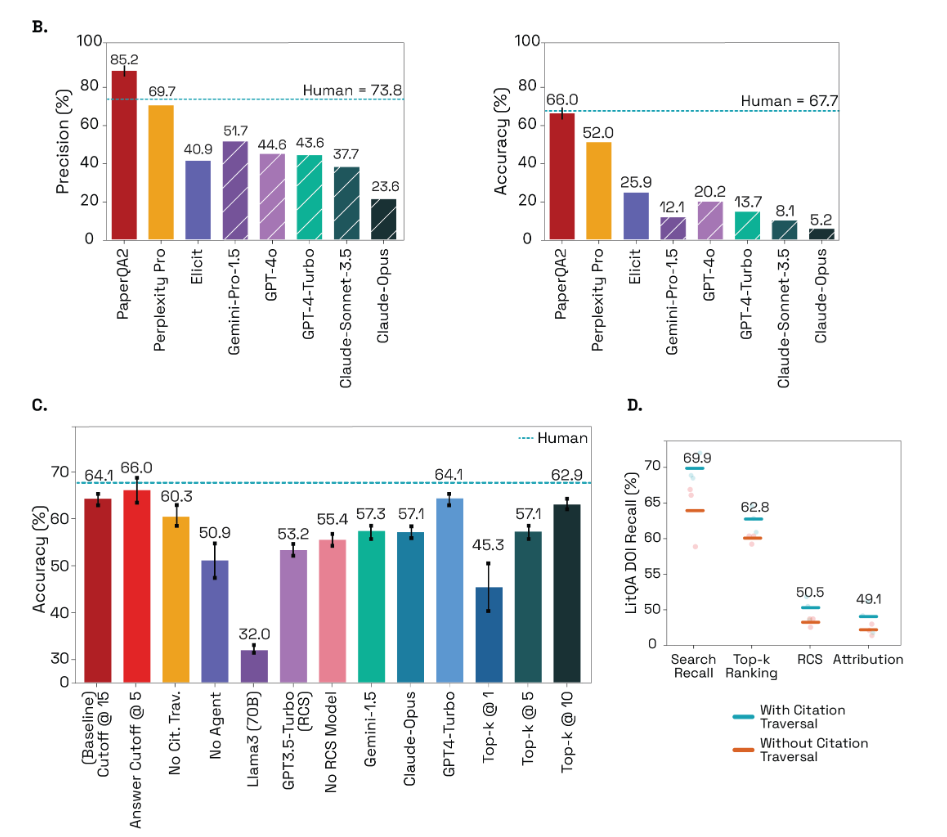
\includegraphics[width=\textwidth]{figures/original_result.png}
    \caption{Original Paper Results. B: Precision and Accuracy of PaperQA and LLMs on LitQA. C: Accuracy of verious abalations of PaperQA. D: Aggragated DOI Recall at each stage (This result is not relevant to this report.)}
    \label{fig:original_result}
\end{figure}

\subsection{RAG vs. Standalone LLM}

Similarly to the paper, the results from this project showed that PaperQA outperforms standalone LLMs in question answering. However, there is a difference in how the LLM attempted to answer the questions. In all of the standalone LLM evalutions, the LLM attempted to answer every single question, and hence the accuraccy and precision was the same for every result, and hence results in a large number of hallucinations, rather than saying that it cannot answer the question. The standalone LLM used in this experiment was \texttt{gpt-4o-mini}, but the standalone LLM used in the original paper was \texttt{gpt-4-turbo}. The performance of 4o-mini is slightly worse in terms of accuracy, but better in terms of precision. 

\subsection{PaperQA Ablations}
The following experiemnts tested the effect of changing key hyperparameters of PaperQA, from the LLM used for the agent and the RAG model to the top-k retrieval and answer cutoff. 

The recreated baseline paperQA uses \texttt{gpt-4o-mini} as the agent LLM, \texttt{gpt-4o-mini} as the RAG model, and a top-k of 30, answer cutoff of 5. The text embedding was the PaperQA default embedding, which is \texttt{text-embedding-3-small}. The original baseline used \texttt{gpt-4-turbo} as the agent LLM, \texttt{gpt-4-turbo} as the RAG model, and a top-k of 30, answer cutoff of 15. 
The reason that the baseline of answer cutoff of 5 was used, was because it was the reuslt that achieved 'superhuman' performance. The recreated baseline seemed to exceed the original baseline, achieving superhuman performance in both accuracy and precision. 

To more similarly recreate the original result, an experiment was run with the PaperQA instead using the \texttt{gpt-4-turbo} agent LLM, and \texttt{gpt-4-turbo} as the RAG model. The expected performance was to be similar to the original result, but in this experiment, superhuman performance was achieved for both the accuracy and precision. Assuming this was an errorneous result, an inspection into the results yielded no such evidence, with the individual results being assigned the correct score for the outputted answer. \\

Strangely, the results showed that using PaperQA with the \texttt{gpt-4.1} as both the agent and the RAG model, the accuracy dropping to sub-human performance compared to the original result and the GPT-4-Turbo result, with the precision being similar, albeit slightly lower. This was an unexpected result as GPT-4.1 is a much newer model that should outperform GPT-4-Turbo in every metric. 

For all of the variations in models being used, the model that performed in terms of accuracy was actually the GPT-4o-Mini model that used the best-in-class text embedding model, Gemini's \texttt{text-embedding-004}. It outperofmred the original baseline, and consistently achieved superhuman performance in both accuracy and precision. \\

Increasing the Answer Cutoff had the same effect as the original paper, decreasing the accuracy, but the effect of removing the RCS step was much less pronounced than the orginal paper, with the original paper showing the accuracy was reduced by 12.8\% compared to the recreated baseline, which was reduced by 6.1\%.\\

The effect of changing the top-k retrieval had a much smaller effect on the accuracy comapred to the original paper. The general trend in the paper was that decreasing the top-k would decrease the accuracy, but the experiments showed there seemed to be no correlation. In fact, lowering the top-k to below 10 still yielded near superhuman performance in accuracy, which the original paper with a top-k of 30 could only just about achieve. 

The interesting result is that all of the experiements involving RAG completely humans out of the water in terms of accuracy, with all of the ablations achieving at least 77.3\% accuracy, and the best performing abalation achieving 89.5\% accuracy, besting the human benchmark of 73.8\%. 

The accuracies of the ablations were much more varied than the precisions, but they did not vary as much as the original paper. All of the RAG models and experiments either were close to or beat human performance, even when given hyperparameters that should have theoretically have hindered performance. 







RCS decreases accuracy and precision but has less of an effect than reducing top k for accuracy. 





